\chapter{Estudi \ac{UX}}

\section{Anàlisi}
L'objectiu d'aquest apartat és definir com seran els usuaris potencials de l'aplicació. Per a fer-ho s'analitzarà com interaccionen amb les aplicacions de gestió de despeses per extreure les necessitats i els requeriments del producte.

\subsection{Investigació contextual}
En aquesta secció s'ha estudiat com els usuaris gestionen les despeses.  Per a fer-ho, s'han enquestat 9 usuaris sobre com gestionen actualment les seves despeses. A més a més, a 4 d'aquests 9 usuaris se'ls ha demanat que utilitzessin varis aplicacions ja existents al mercat (\gls{Google_play}). Un cop la feien servir en directe se'ls preguntava quines coses els havien agradat i quines no. 

La totalitat de l'entrevista ha estat transcrita al moment i conduida per la plantilla de la figura \ref{fig:plantilla_analisi}. És important remarcar que tot i ser una entrevista es buscava, sempre que era possible, que els usuaris mostressin com treballen, enlloc de que expliquessin amb paraules com ho fan. També, quan els usuaris utilitzaven les aplicacions s'ha gravat un vídeo amb el que veien a la pantalla mentre feien servir les aplicacions així com el que poguessin estar dient en aquell moment. L'objectiu de fer aquestes gravacions és facilitar, si s'escau, el posterior anàlisi per aclarir parts de l'enquesta que no fossin prou clars. Al comptar amb so, també ha servit per localitzar i identificar les funcions o apartats que frustraven o motivaven als usuaris. Per últim, quan ha estat possible s'han recol·lectat imatges o documents que ensenyessin com els usuaris gestionen les seves despeses i/o ingressos. 

\begin{figure}[htp]
\centering
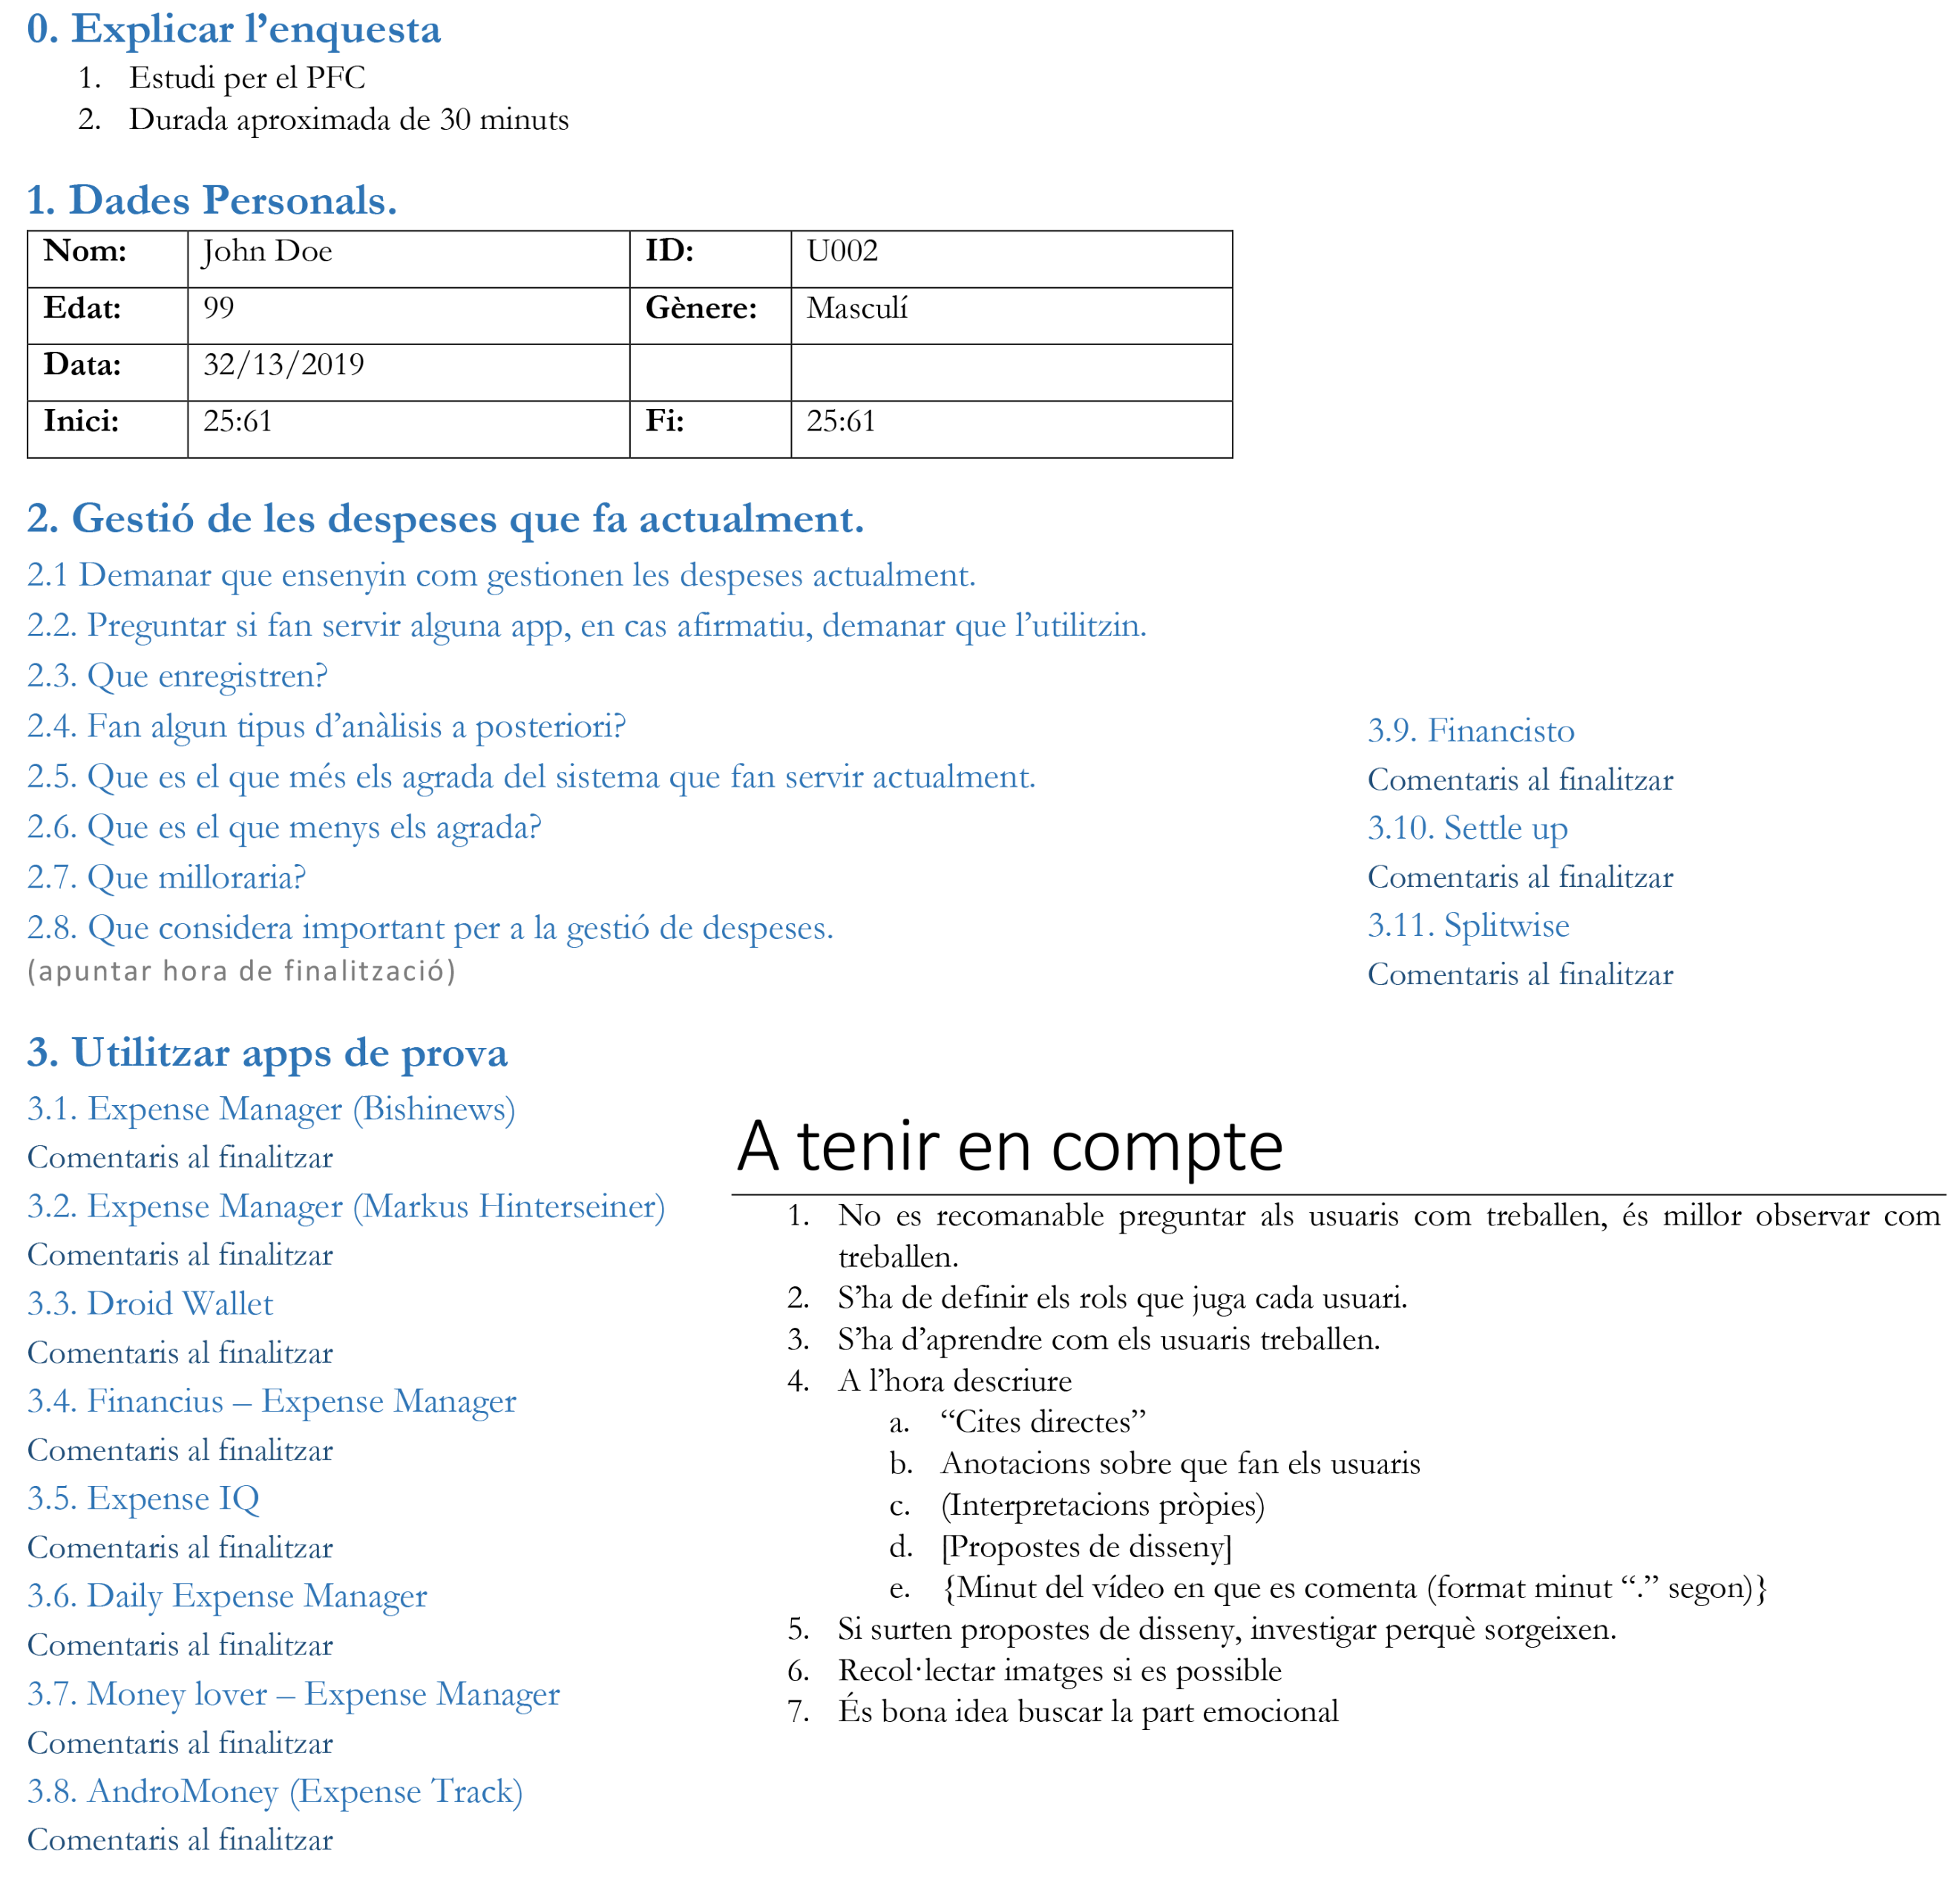
\includegraphics[scale=0.75]{plantilla_analisi.png}
\caption{Plantilla emprada a la investigació contextual}\label{fig:plantilla_analisi}
\end{figure}

\subsection{Anàlisi contextual}
%TODO Work roles
%TODO Flow model

\begin{figure}[htp]
\centering
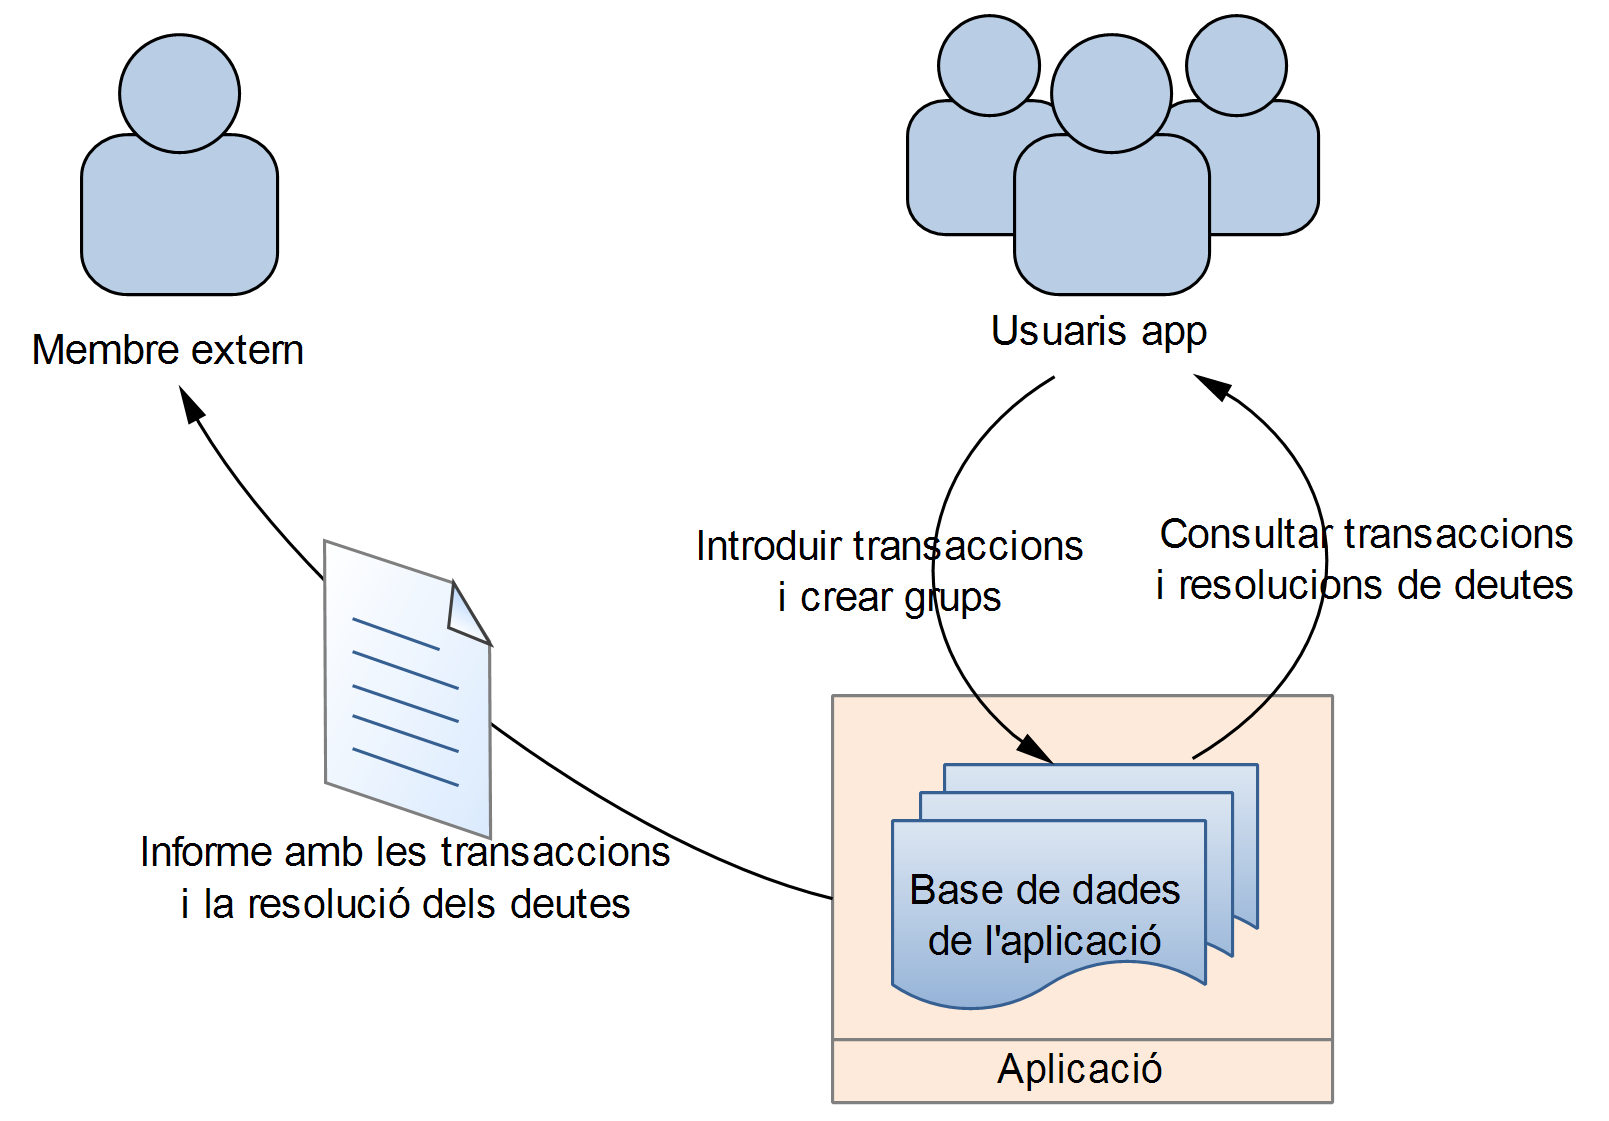
\includegraphics[scale=1]{flow_model.png}
\caption{Model de flux}\label{fig:flow_model}
\end{figure}